% =====================================================================
\appendix
\section{AES Block-Size Sweep (detailed values)}
\label{app:blocksize}

Table~\ref{tab:blocksize} gives the full per-size measurements behind the offload-weight curve of
Figure~\ref{fig:weight}, all on a real GPU on an \emph{idle} device (no co-tenant compute), driving a
single-event-loop server (Python \texttt{asyncio} with a 32-thread executor) at 50 concurrent
clients. The AES block size is swept over consecutive powers of two from $4$\,KiB (launch-bound,
tens of microseconds) to $8$\,MiB (bandwidth-bound, $\sim$$2.3$\,ms). For each we report the
measured single-op GPU latency (one offload in flight), the synchronous and asynchronous
throughput, and their ratio; \S\ref{sec:eval} interprets the curve.

\begin{table}[h]
  \centering
  \begin{tabular}{rrrrr}
    \toprule
    block size & GPU latency (\textmu s) & sync (req/s) & async (req/s) & speedup \\
    \midrule
    4\,KiB   & 46.4   & 3750 & 4667 & $1.24\times$ \\
    8\,KiB   & 47.0   & 3688 & 4650 & $1.26\times$ \\
    16\,KiB  & 51.4   & 3657 & 4573 & $1.25\times$ \\
    32\,KiB  & 60.3   & 3501 & 4371 & $1.25\times$ \\
    64\,KiB  & 70.2   & 3326 & 4355 & $1.31\times$ \\
    128\,KiB & 92.7   & 2970 & 4218 & $1.42\times$ \\
    256\,KiB & 126.5  & 2706 & 4128 & $1.53\times$ \\
    512\,KiB & 191.8  & 2454 & 4494 & $1.83\times$ \\
    1\,MiB   & 361.6  & 1538 & 3644 & $2.37\times$ \\
    2\,MiB   & 653.6  & 966  & 2858 & $2.96\times$ \\
    4\,MiB   & 1188.1 & 506  & 1937 & $3.83\times$ \\
    8\,MiB   & 2258.6 & 227  & 1228 & $5.41\times$ \\
    \bottomrule
  \end{tabular}
  \caption{Real-GPU AES block-size sweep on a single-event-loop server (idle GPU). Source:
    \texttt{transparent-runtime/apps/aes\_blocksize\_py\_results.csv}.}
  \label{tab:blocksize}
\end{table}


% =====================================================================
\section{Interposition Obstacles for the Transparent Runtime}
\label{app:obstacles}

Running stock binaries under the \texttt{LD\_PRELOAD} fiber runtime of \S\ref{sec:transparent}
surfaced five obstacles below the architectural walls. Each was resolved once and is recorded here
because any threading-interposing tool will meet them.

\paragraph{The condition-variable versioning hazard.}
The sharpest obstacle is a \emph{symbol-versioning} hazard~\citep{drepper}: the glibc
condition-variable functions carry two incompatible ABIs under one name
(\texttt{GLIBC\_2.2.5} and \texttt{GLIBC\_2.3.2}), so a naive interposer that defines an
\emph{unversioned} \texttt{pthread\_cond\_signal} breaks the linker's version-matched relocation
and silently corrupts \emph{some} binaries while sparing others: in our sweep it crashes MariaDB
at startup with a wild pointer and is tolerated by Redis, memcached, nginx, and stunnel
(Figure~\ref{fig:condsweep}). Because a transparent runtime cannot know in advance which binaries
are susceptible, version-matched interposition is mandatory: export the interposed symbols at
their exact version via a linker version script and resolve the real ones with \texttt{dlvsym}.

\begin{figure}[h]
  \centering
  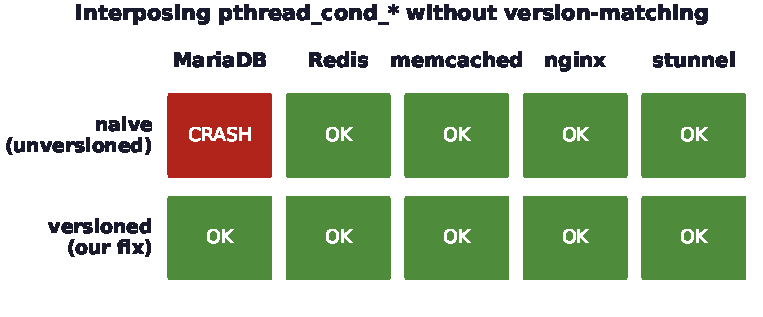
\includegraphics[width=0.9\linewidth]{figs/fig_condsweep.pdf}
  \caption{A reusable interposition hazard. The glibc condition-variable functions carry two
    incompatible ABIs under one name. A naive unversioned interposer breaks the version-matched
    relocation and silently corrupts \emph{some} binaries (MariaDB crashes at startup) while
    sparing others. Version-matching the interposed symbols fixes all of them.}
  \label{fig:condsweep}
\end{figure}

\paragraph{Four lesser obstacles.}
\begin{itemize}[leftmargin=1.4em,itemsep=2pt,topsep=2pt]
  \item \textbf{Alternate I/O entry points.} A server may do its socket I/O through
    \texttt{recv}/\texttt{send}/\texttt{poll} rather than \texttt{read}/\texttt{write}, so every
    blocking entry point the application can reach must be interposed to yield the fiber.
  \item \textbf{Real-thread identity.} \texttt{pthread\_self} must return the genuine OS thread
    identity, because the C library's stack-bounds logic relies on it; returning a per-fiber value
    breaks libc internals.
  \item \textbf{Carrier re-establishment after \texttt{fork}.} A daemon that forks drops the carrier
    thread in the child; the carrier must be re-established before any fiber can run.
  \item \textbf{Priority inversion.} Pinning the carrier to a real-time priority can invert priorities
    against a lock holder running at normal priority, stalling the carrier.
\end{itemize}
